% --------------------------------------------------------------------------------------------------
\section{Exploratory Data Analysis}

% --------------------------------------------------------------------------------------------------
\subsection{Outliers}
Figue \ref{figure_dataset} (left) presents the datasets and show several unusual down spikes that 
could be considered as outliers (\textit{e.g.} with an electricity consumption lower than 120 kW). 
These values are remplaced by the average value of electricity consumption (see figure 
\ref{figure_dataset} right and R code below). Some statistics of the dataset are presented in table 
\ref{table_dataset}.


\begin{lstlisting}[language=R]
meani = mean(as.numeric(unlist(data[1:nrow(data),"Power (kW)"])), na.rm=TRUE)
for (index in which(z[,"Power (kW)"]<120))
  {data[index,"Power (kW)"] = meani}
\end{lstlisting} 

\begin{figure}[H]
\centering
 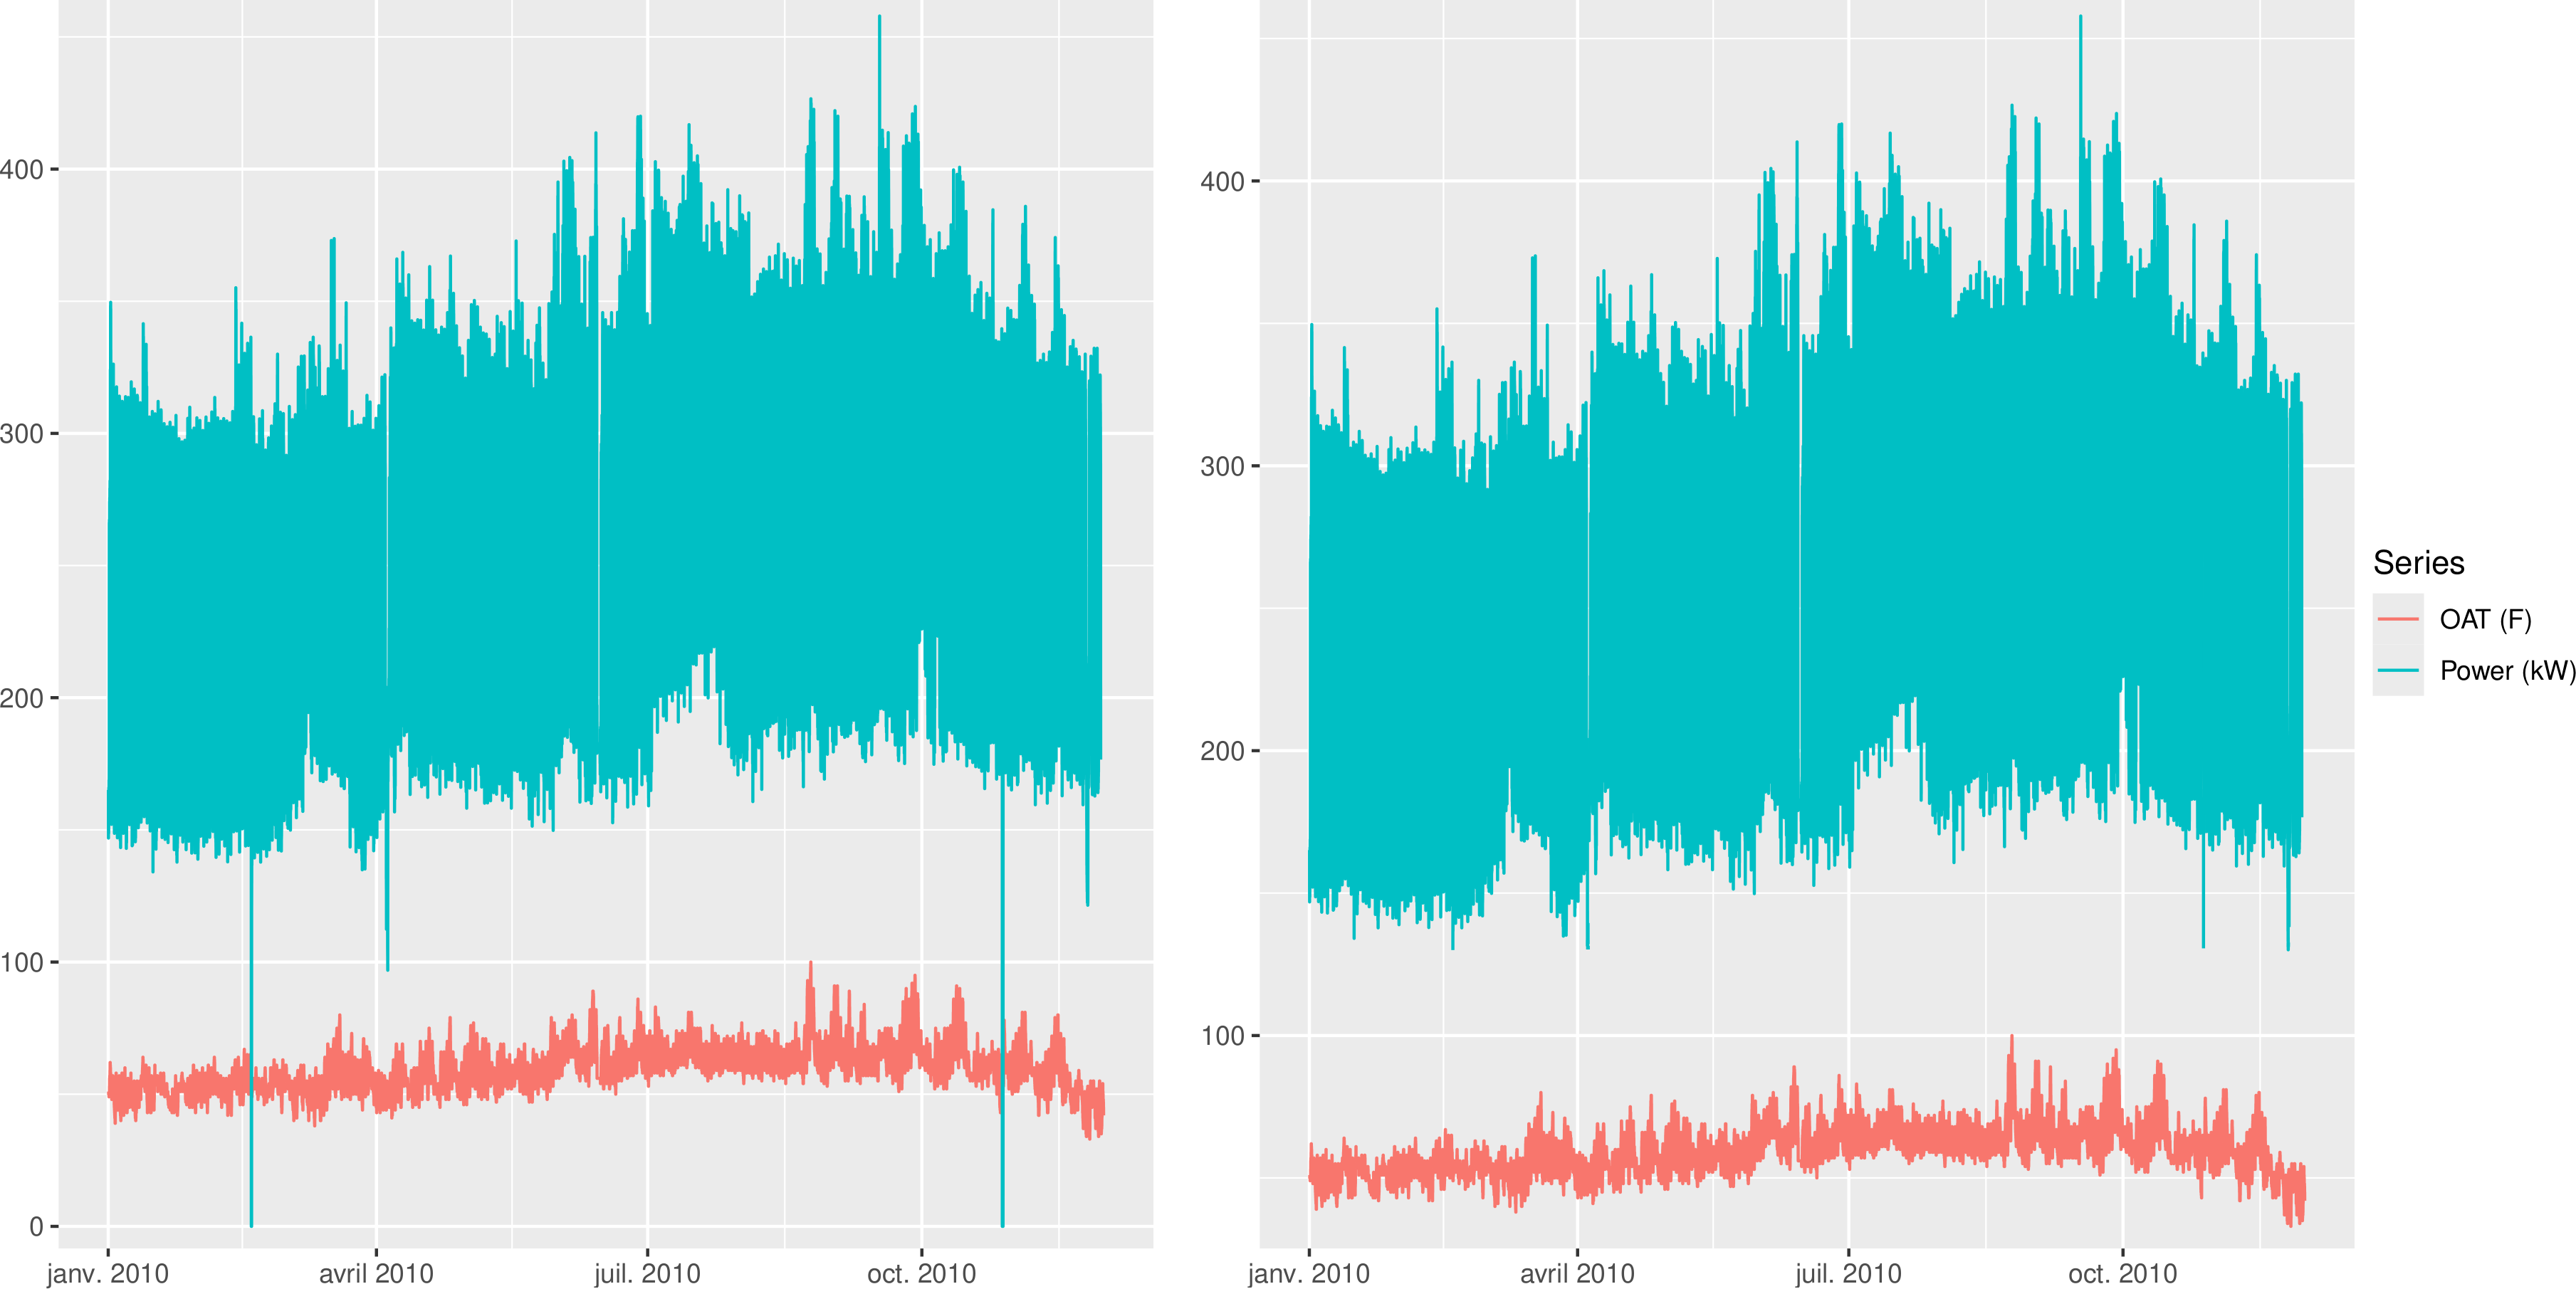
\includegraphics[scale=0.4]{figures/dataset.png}
\caption{Original dataset (left) and dataset with removed outliers (right).}
\label{figure_dataset}
\end{figure}

\begin{table}[H]
\centering \begin{tabular}{c|ccccc}
 & \textbf{Minimum} & \textbf{Maximum} & \textbf{Mean} & \textbf{Median} & \textbf{Variance} \\ \hline
\textbf{Power (kW)} &  0.0 & 457.9 & 262.3 & 276.5 & 66.0 \\
\textbf{OAT (F)}    & 33.0 & 100.0 &  59.0 &  58.0 & 8.8 \\
\end{tabular}
\caption{Basic statistics of the dataset.}
\label{table_dataset}
\end{table}


% --------------------------------------------------------------------------------------------------
\subsection{Trend and seasonality}
Using moving averages, the \texttt{decompose} R function returns the trend and seasonal components 
of the time series. Figure \ref{figure_decompose} presentes the components of the electricty power 
time series. 

\begin{figure}[H]
\centering
 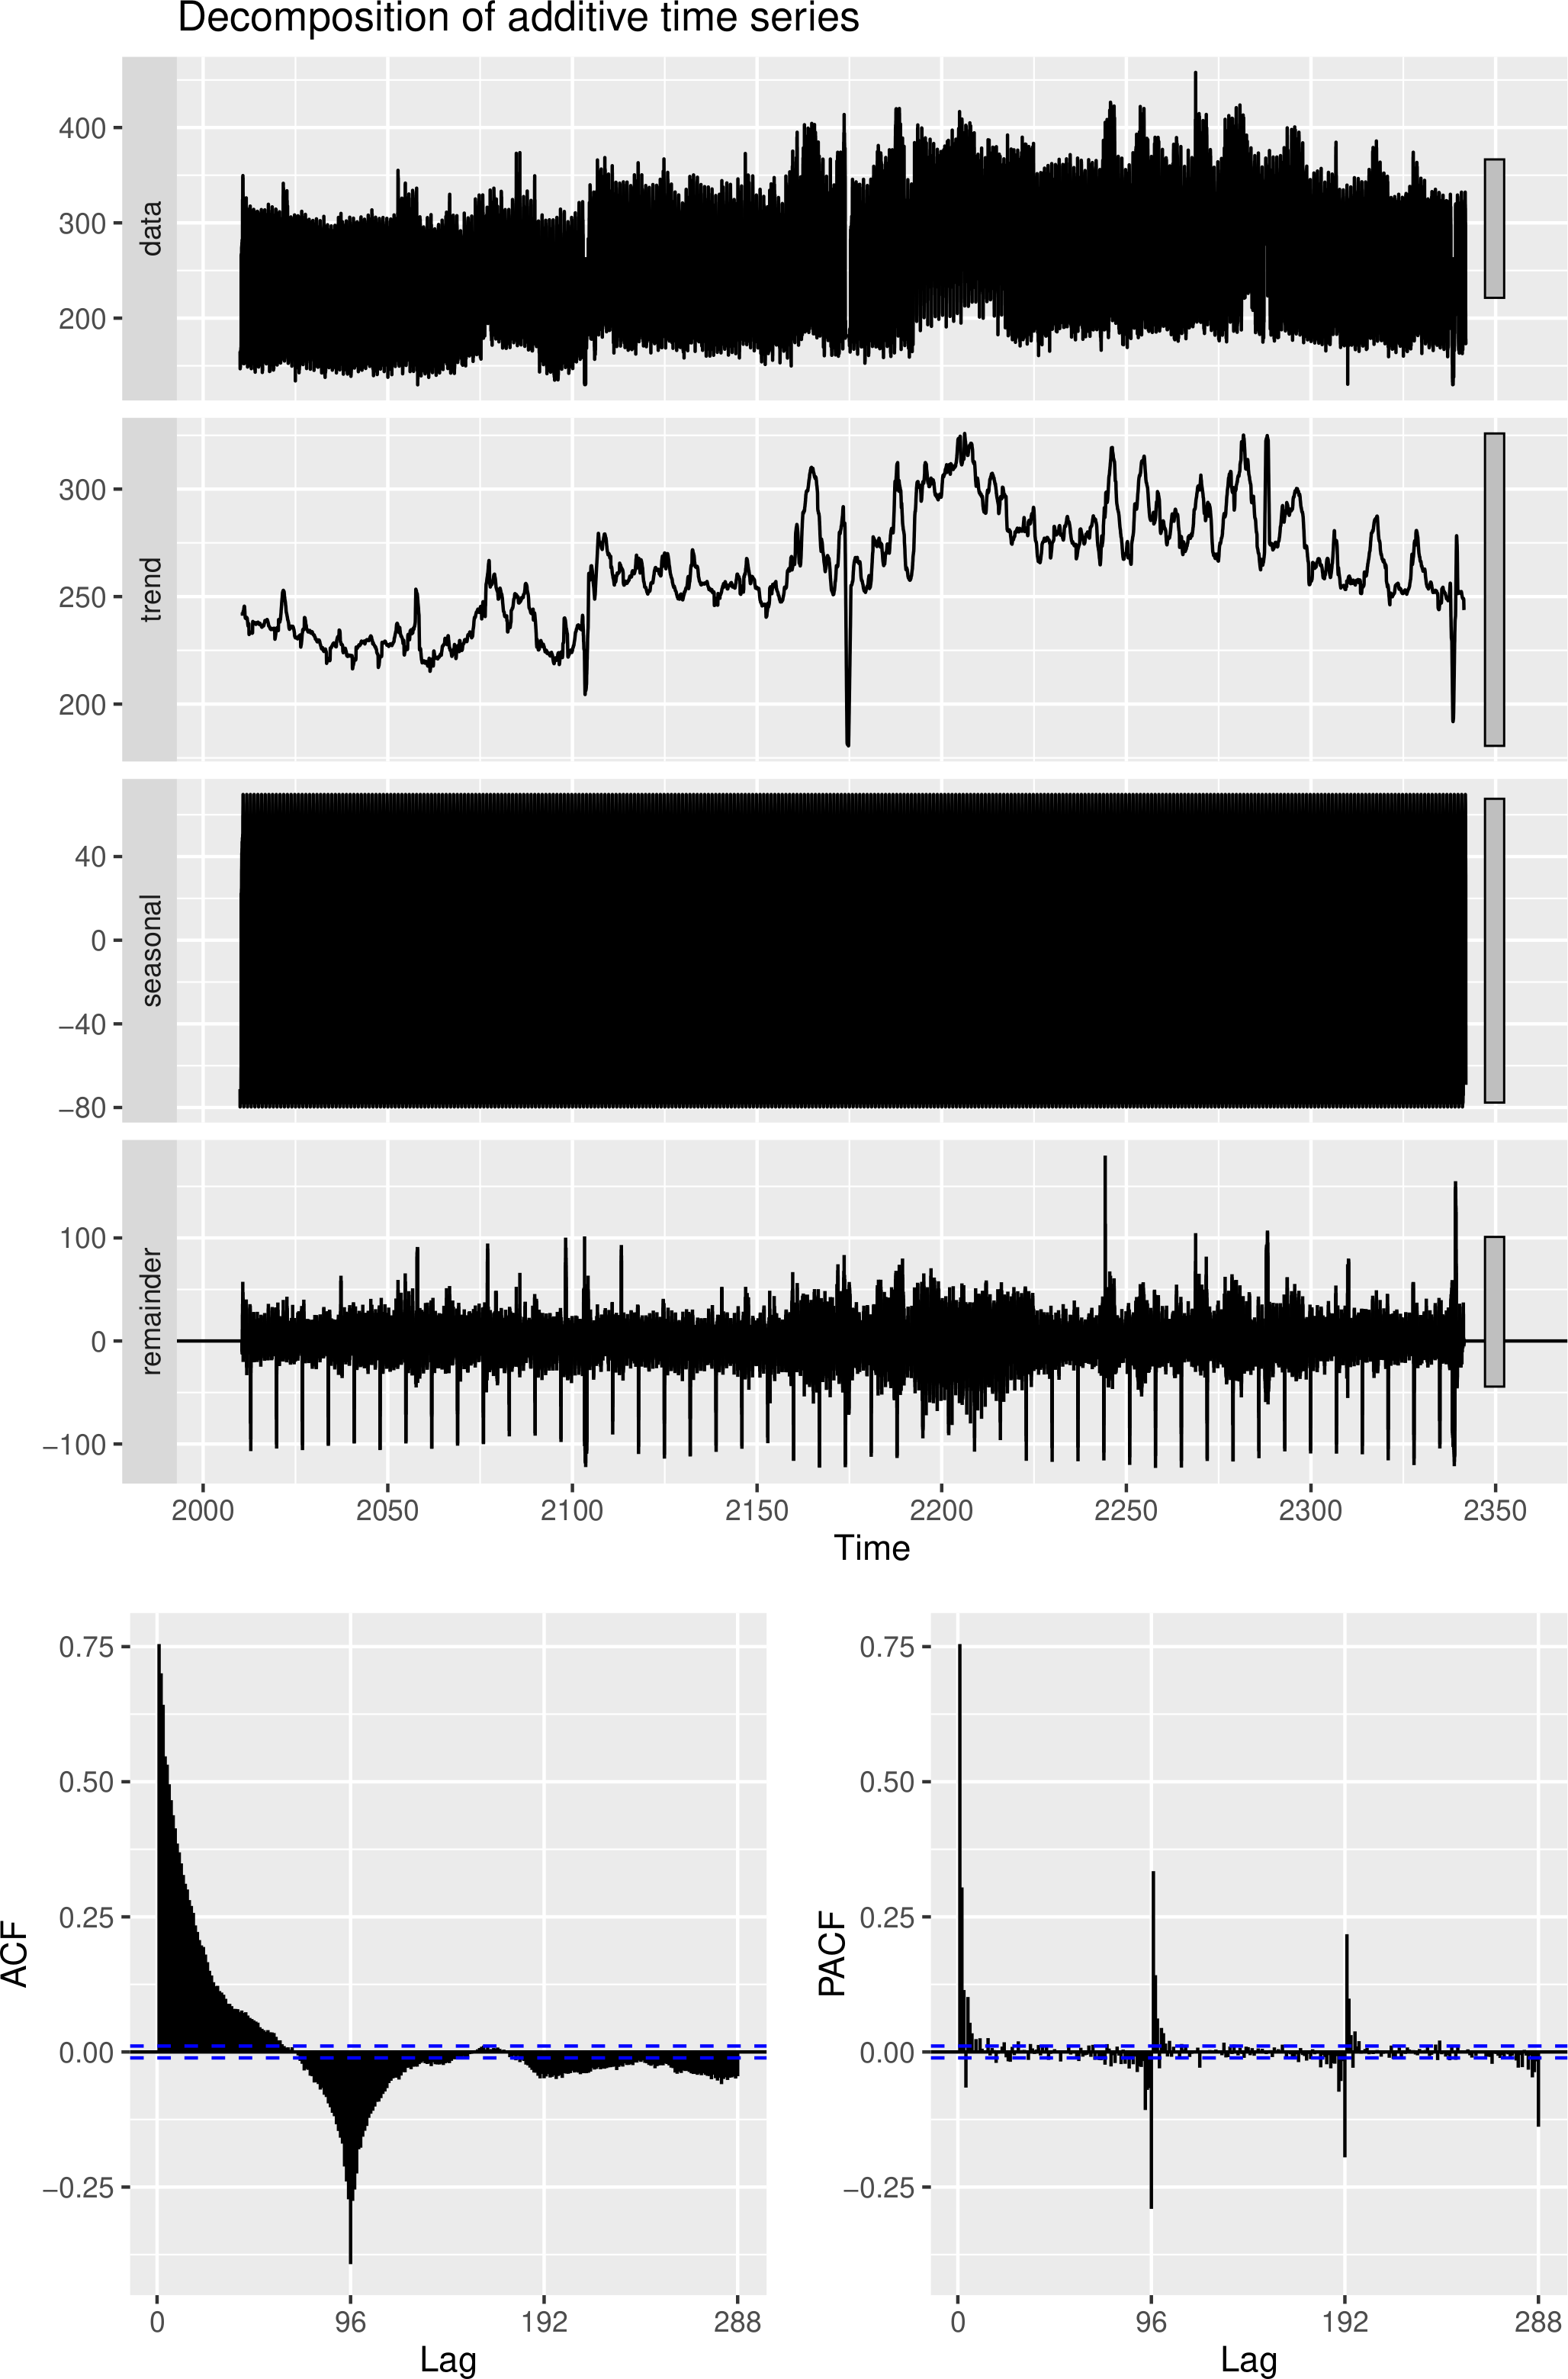
\includegraphics[scale=0.45]{figures/decompose.png}
\caption{Trend and seasonal components of the electricity consumption time series.}
\label{figure_decompose}
\end{figure}

The decomposition shows linear trend that varies in time (figure \ref{figure_decompose} TREND and 
ACF frames) and a significant seasonality of 96 lag (figure \ref{figure_decompose}, PACF frame) that 
corresponds to one day.

% --------------------------------------------------------------------------------------------------
\subsection{Noise}
The remainder of the decomposition of the electricity power time series (figure 
\ref{figure_decompose} REMAINDER frame) shows periodic fluctuations with relatively large 
amplitudes. These patterns seems to imply multi seasonality.

% --------------------------------------------------------------------------------------------------
\subsection{Covariate}
The cross-correlation test (see R code below) that test the zero-correlation between the 
electricity power time series and the covariate Outdoor Air Temperature show p-values always null. 
We reject the null hypothesis, there is no zero correlation. In other words, there is high 
correlation between the two variables. Because of this high correlation, the covariate data might 
no convey additional information. Using covariates for modelling and forecasting might not be 
significant. In this analysis modelling and forecasting is done with and without the covariate for 
comparison.

\begin{lstlisting}[language=R]
cc.test(data[,"OAT (F)"], data[,"Power (kW)"], max.lag=10, plot=FALSE) 
\end{lstlisting}
